% This is samplepaper.tex, a sample chapter demonstrating the
% LLNCS macro package for Springer Computer Science proceedings;
% Version 2.21 of 2022/01/12
%
\documentclass[runningheads]{llncs}
%
\usepackage[T1]{fontenc}
% T1 fonts will be used to generate the final print and online PDFs,
% so please use T1 fonts in your manuscript whenever possible.
% Other font encondings may result in incorrect characters.
%
\usepackage{graphicx,rotating}
% Used for displaying a sample figure. If possible, figure files should
% be included in EPS format.
%
% If you use the hyperref package, please uncomment the following two lines
% to display URLs in blue roman font according to Springer's eBook style:
%\usepackage{color}
%\renewcommand\UrlFont{\color{blue}\rmfamily}
%\urlstyle{rm}
\usepackage[hidelinks]{hyperref}
\usepackage{multirow}
\begin{document}
%
\title{Enhancing End-to-End Malayalam Automatic Speech Recognition with Language Model Augmentation}


\titlerunning{Malayalam ASR with Language Model}
% If the paper title is too long for the running head, you can set
% an abbreviated paper title here
%
% \author{Kavya Manohar\inst{1}\orcidID{0000-0003-2402-5272} \and
% Ashish Abraham\inst{2}\orcidID{} \and
% Gokul G Menon\inst{3}\orcidID{}}
% %
% \authorrunning{K. Manohar et al.}
% % First names are abbreviated in the running head.
% % If there are more than two authors, 'et al.' is used.
% %
% \institute{Digital University Kerala, India \\
% \email{kavya.manohar@duk.ac.in} \and
% Ashish Address \\
% \email{ashishabraham22@gmail.com}\\
% % \url{http://www.springer.com/gp/computer-science/lncs}
% \and
% Gokul Address\\
% \email{gokulgmenon@gmail.com}}
%
\maketitle              % typeset the header of the contribution
%
\begin{abstract}

Self-supervised learning (SSL) representations using transformers from multilingual speech have significantly improved the performance of automatic speech recognition (ASR) tasks in low-resource languages. This study focuses on the development of an ASR system for the Malayalam language using pretrained SSL representations and enhance its performance with the inclusion of a statistical n-gram language model. Our findings indicate that this language model augmentation reduces the word error rate by 12.5\% on in-domain test data and 5.9\% on out-of-domain test data. The datasets used are diverse, encompassing a variety of speakers, speech domains, and recording environments.  Our results underscore the critical role of augmenting pre-trained speech representations with language models in developing ASR systems for languages with limited training resources. The model is made openly available on HuggingFace for reproducibility and adaptation to similar languages.
% We compare the outcomes of fine-tuning transformer-based models with traditional speech recognition methods, where acoustic and language models are trained separately and then integrated. The resulting word error rates vary significantly depending on the test dataset.
 
\keywords{Self-supervised Learning  \and Speech Recognition \and Pretrained Models \and Low-resource language \and Language Model \and Malayalam}
\end{abstract}

\section{Introduction}

Self supervised learning (SSL)  representation for speech has proven to be effective in diverse speech tasks including speech recognition, classification and even translation \cite{baevski2020wav2vec,babu2021xls,barrault2023seamlessm4t}.  They are built on the idea proposed in \cite{schneider2019wav2vec} where a generic representation of speech can be computed from a huge of unlabelled speech corpus in a process called pre-training. This multi lingual speech representations learnt from huge collection of unlabelled data has proven to be effective in building automatic speech recognition (ASR) systems for languages with limited annotated corpora \cite{conneau2020unsupervised}. Alternately there are sequence to sequence architectures like Whisper \cite{whisper} that uses weakly supervised pre-training on multilingual corpora followed by language specific fine-tuning to achieve comparable performance on ASR tasks. These transformer based ASR models can work even without explicit language modelling that has been conventionally an essential component in hybrid ASR systems \cite{manohar2023automatic}.

In this paper we present the results of fine-tuning the XLS-R model \cite{babu2021xls} of 300 million parameters using publicly available Malayalam read speech corpora. We augment this process with an explicit statistical language modelling using publicly available Malayalam text corpora. We test the resulting ASR model on different test datasets, including out of domain (OOD) speech data. The results are compared with the finetuned models without an explicit language model.
% We also study the impact of using language model adaptation to improve ASR performance. 




% Automatic Speech Recognition (ASR) is the process of converting natural human speech to textual form. Conventionally, an ASR system is built by combining (i) an acoustic model trained on an labelled speech corpus (ii) a language model trained on textual data and (iii) a pronunciation lexicon, that describes the pronunciation of a list of words that are ought to be recognised by the ASR. This is referred to as a hybrid ASR architecture and described in Fig.~\ref{asr}.

% \begin{figure}
%     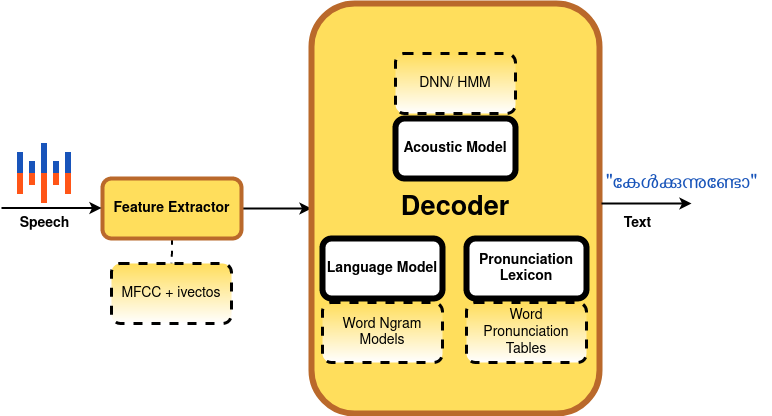
\includegraphics[width=\textwidth]{ASR.png}
%     \caption{Architecture of a conventional hybrid ASR} \label{asr}
% \end{figure}

% 


% Closely following the popular Wav2Vec \cite{baevski2020wav2vec} architecture, pre-trained cross-lingual speech representations for Indic languages have also been reported \cite{gupta2021clsril}. The recent cross lingual speech representation (XLS-R) architecture uses 436K hours of publicly available unlabelled speech data from 128 languages to  prepare pre-trained neural speech representation models \cite{babu2021xls}. Our work is an attempt to utilise the capabilities of modern pre-trained audio transformers to build end-to-end speech recognition systems for low-resource languages like Malayalam.

% In this paper we present the results of fine-tuning the XLS-R model of 0.3B parameters with a Ken language model using publicly available Malayalam read speech corpora. We test the resulting ASR model on different test datasets, including out of domain (OOD) speech data.
% % We also study the impact of using language model adaptation to improve ASR performance. 
% The results are compared with the baseline models developed using conventional hybrid ASR architecture. 

% We have not attempted the integration of a language model after the fine-tuning process, but it is planned as a future work.

\section{Related Works}
\label{sec:relatedworks}

The development of modern End-to-end ASR systems has been made possible by neural architectures, which enable the integration of different components of the system, including the acoustic model, language model, and pronunciation lexicon model, into a single network \cite{georgescu2021performance}. 
In the past  few years, several  techniques have been proposed to overcome the challenges of limited speech resources in building end-to-end ASR systems \cite{barrault2023seamless,pratap2024scaling,whisper} .
% This often requires tens of thousands of hours of labelled speech data for training than conventional hybrid ASR systems \cite{bayerl2019comparison}. 


\begin{figure}[htpb]
    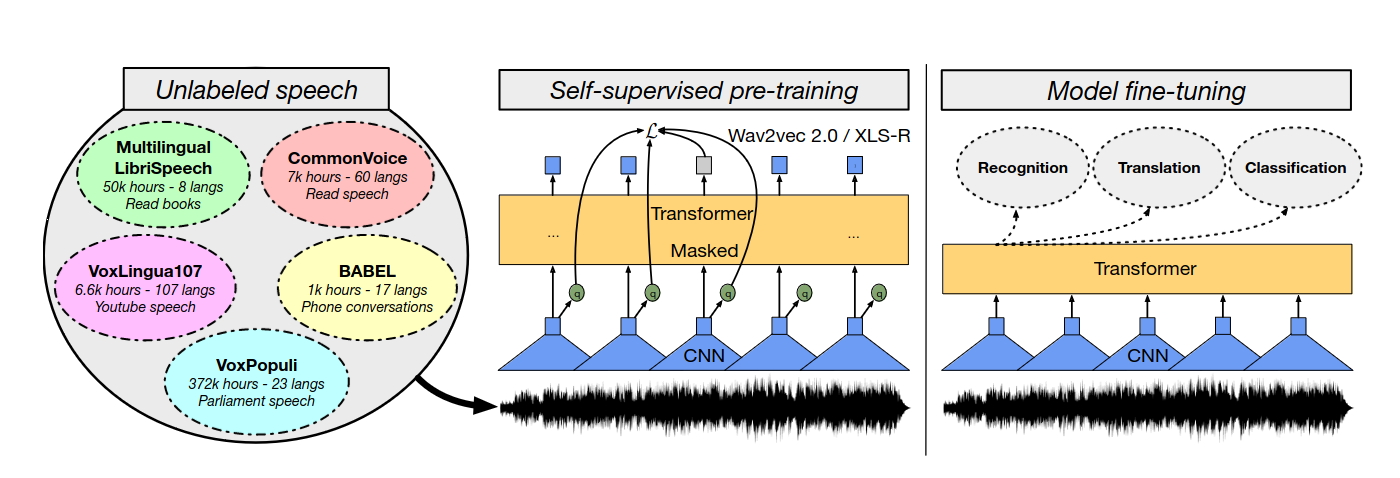
\includegraphics[width=\textwidth]{XLS-R.png}
    \caption{The Self-supervised learning architecture XLS-R \cite{babu2021xls}.} \label{XLS-R}
\end{figure}


Self-supervised learning (SSL) is one such technique where in, a neural speech representation model is trained utilising a lot of unlabelled data  \cite{schneider2019wav2vec,baevski2020wav2vec,conneau2020unsupervised,barrault2023seamlessm4t}. This is referred to as pre-training. On top of the speech representation, a small labelled corpus can be used to achieve any supervised tasks such as speech recognition, emotion recognition, speaker identification and language identification. The number of languages used for pretraining vary from 53 languages in XLSR to 1107 languages in MMS \cite{pratap2024scaling}. In a procedure known as fine-tuning, the pre-trained model can be adapted with comparably less amount of labelled data for a specific task like speech recognition, emotion recognition as indicated in Fig. \ref{XLS-R}. For ASR, fine-tuning relies on the connectionist temporal classification (CTC) algorithm, which maps speech representations learnt during pre-training to the character sequences of the transcription script \cite{georgescu2021performance}.

An alternate approach is to build an End-to-end ASR using the sequence to sequence transformer training in a weakly supervised manner. Here huge labelled speech corpora is needed and the most popular implementation of this approach is the Whisper model which is pretrained on 680 thousand hours of multilingual labelled speech data\cite{whisper}. The Whisper architecture predicts  text tokens in its output. The Whisper model provides various pre-trained checkpoints for fine-tuning with additional labelled speech data for improved ASR performance.

Recently, there have been increased efforts to collect and document more Indian language speech corpora, which are then used to train additional pre-trained checkpoints such as IndicWhisper \cite{bhogale2023vistaar} and IndicVoices \cite{javed2024indicvoices}. Prior to this, attempts were made to enhance the performance of unified ASR for Indian languages by incorporating multilingual language models in the SLP1 writing scheme \cite{anoop2022}, building on top of Indic Wav2Vec \cite{javed2022towards}. However, there has been limited progress in incorporating an additional monolingual language model to improve End-to-End ASR performance in the Malayalam language using the native script. In contrast, in hybrid ASR systems, the language model is an essential component. Results from using statistical n-gram language models with various subword units, ranging from syllables to words in Malayalam in hybrid ASR models have been reported in \cite{manohar2023improving}.


% \textit{The pre-training finetuning concept in Whisper, Wav2Vec, XLS-R}

% \textit{Attempts to finetune them. Vistaar. Indic Wav2Vec, Anoop CS work}

% \textit{Other Malayalam ASR work - Kavya.}

% \textit{Any prior work on LM adaptation on top of Wav2Vec or Whisper}

% \textit{Types of Language Modelling, KenLM. Characetr LM, word LM and subword LM \cite{ahmed-2023-improving}}

% There are numerous works that attempted to solve various challenges associated with Malayalam ASR. A universal comparison of results is not possible due to the unavailability of publicly available baseline test dataset in Malayalam. Out of vocabulary (OOV) words largely affect the WER, and most of the reported works use private datasets to train and test the ASR models, which does not detail the OOV rates of test datasets.

% \subsection{Conventional hybrid ASR}

% One of the earlier work on recognising continuous Malayalam speech uses HMM-ANN architecture and reports a WER of 13\% \cite{mohamed2012hmm}. An automatic phonetic recognizer for continuous Malayalam speech, trained on manually aligned phonetic transcription of waveforms  has resulted in a phonetic engine with recognition accuracy of 40.93\%  \cite{thennattil2016phonetic}. %when tested on 1 hour 15 minutes of speech. 
% A work on continuous Malayalam speech recognition using CMU Sphinx toolkit with semi-automatically transcribed phonetic lexicon and GMM-HMM acoustic model has reported a sentence recognition accuracy of 84\% \cite{kurian2015development} and another work on similar lines has reported a WER of 34.8\% \cite{deekshitha2018development}. Recently, there has been many reported works on continuous Malayalam speech recognition using Kaldi toolkit \cite{povey2011kaldi}, employing advanced acoustic modelling like GMM (LDA+MLLT+SAT) \cite{babu2018continuous}, SGMM \cite{lekshmi2021asr}, DNN \cite{moncy2020automatic} and TDNN \cite{kavya2022}.

% \subsection{End-to-end ASR}

% There has not been much explorations on end-to-end ASR architectures for Malayalam ASR due to unavailability of labelled training data. With the advent of SSL models, it has now become possible to fine-tune them effectively even in the context of low resource languages \cite{yi2020applying,holla2022end}. In a previous attempt to fine-tune an ASR model for Malayalam\footnote{\href{https://huggingface.co/gvs/wav2vec2-large-xlsr-malayalam}{Hugging face model}}, a WER of 28\% was reported. It used XLSR-Wav2Vec2.0 transformer that was pretrained on speech data from 53 languages \cite{baevski2020wav2vec}. 

In the proposed work presented in this paper we fine-tune the XLS-R pretrained transformer model using Malayalam read speech corpora from diverse sources as done in \cite{manohar2023automatic} and expand it with language model augmentation during decoding for improved ASR performance. 
% We also compare the results with a hybrid ASR architecture trained and tested on the same datasets. 


\section{Methodology}



The experimental methodology involves fine-tuing a pretrained cross lingual speech representation (XLS-R) model shown in Fig. \ref{finetune}. The first component of the model is a stack of CNN layers that can extract a compressed latent representation, $\mathcal{Z}$, from speech $\mathcal{X}$ \cite{babu2021xls}. They are acoustically meaningful but contextually independent representations. The latent features are continuous and they are quantised to $\mathcal{Q}$, using a quantisation codebook. According to \cite{babu2021xls}, this layer has undergone sufficient training and hence are kept frozen during the fine-tuning process.

\begin{figure}[!h]
    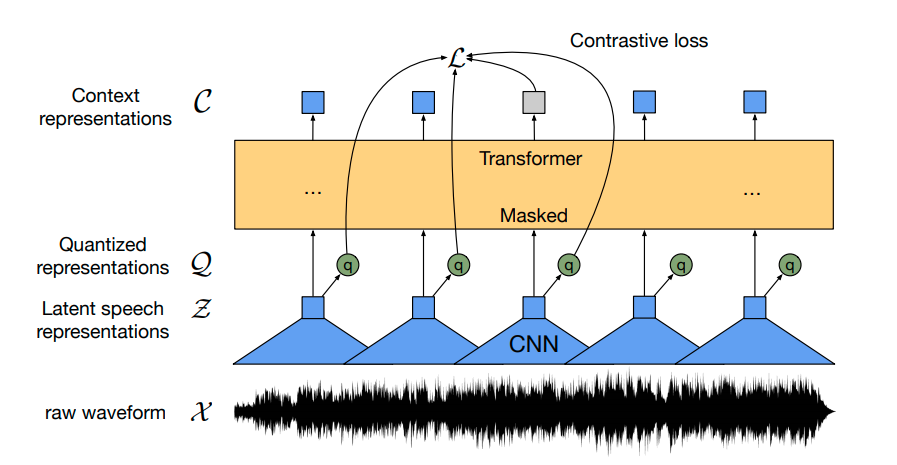
\includegraphics[width=0.8\textwidth]{xlsr.png}
    \centering
    \caption{The pretraining and finetuning steps in XLS-R} 
    \label{finetune}
\end{figure}


The CNN layers are followed by a transformer layer with self-attention. They build contextualised speech representations, $\mathcal{C}$ from the input features $\mathcal{Z}$. The model learns to understand speech patterns by solving a contrastive predictive coding (CPC) problem. This involves identifying the correct quantized speech representation for a masked time step from a set of distractors \cite{babu2021xls}. The pretrained transformer model we use has been trained on unlabelled speech data from 128 languages with a total of 436K hours of publicly available corpora, including Malayalam \cite{babu2021xls}.



% \subsection{Fine-tuning for ASR task}

The purpose of fine-tuning is to map the context representations generated by the pre-trained model to their corresponding character tokens as labels, using labeled speech data. The process of fine-tuning the pre-trained model involves adding a linear classification layer on top of the Transformer and training the entire model by minimising the connectionist temporal classification (CTC) loss. During this process, the quantisation module is disabled and the model learns to map the context representations to the corresponding character tokens as labels. The training is done using the CTC loss, which is a commonly used loss function in ASR systems \cite{graves2006connectionist}. The CTC loss ($\mathcal{L}_{CTC}$) is a mathematical expression defined as in equation \ref{eq:ctcloss}. Here $w^*$ represents the ground-truth transcript, which is a character sequence.

\begin{equation}
\label{eq:ctcloss}
% \vspace{-0.4cm}
    \mathcal{L}_{CTC} = -log \sum_{\pi \epsilon B^{-1}(w^{*}_{1:N})}{\prod_{t=1}^{T}p(\pi_t|c_t)}
\end{equation}

where, T is the number of frames,  N represents the number of character tokens, B is a function to map an alignment sequence $\pi_{1:T}$ to character sequence $w^{*}_{1:N}$, its inverse function $B^{−1}(w^*)$ refers to all the CTC paths mapped from $w^*$ to $\pi_{1:T}$ . The calculation of $p(\pi_t|c_t)$ is performed using the CTC linear layer is followed by a softmax function \cite{graves2006connectionist,ou2022towards}.
% We use this loss function in the fine-tuning step described in section \ref{sec:CTCtuning}.

\subsection{Decoding with a Language Model}

The XLS-R model explained in the previous section serves as an acoustic model. It can predict character probabilities for each time slice. The CTC beam search algorithm converts a series of character probabilities to decoded characters which serve as the ASR output \cite{graves2006connectionist}. This output however is guided by acoustic model alone, which leads to linguistically invalid character sequences or words at the output resulting in high word error rates. But a word level language model (LM) can be augmented to help the decoding process. A statistical LM predicts the conditional likelihood $p(w_{i+1}|w_0 , w_1 , ...w_i )$ of the next word $w_{i+1}$ given the previous words. However with the Markovian assumption that only previous $n$ words are only relevant for the prediction of the next word, we stick to n-gram LM, here $n=3$. The overview of the proposed model is shown in Fig. \ref{Fig:LM-model}.

\begin{figure}[htpb]
    
    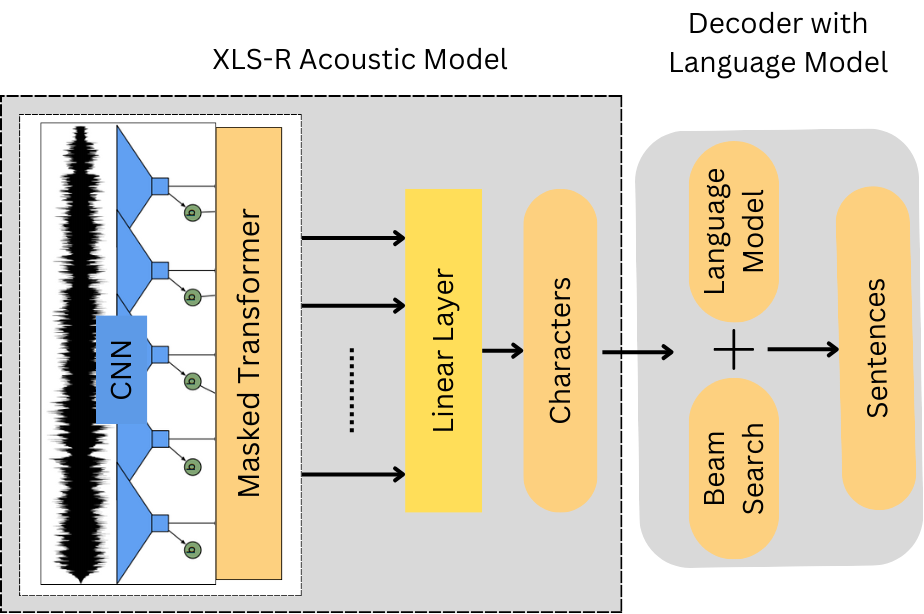
\includegraphics[width=0.7\textwidth]{LM-decoder.png}
    \centering
    \caption{Proposed Architecture to integrate Malayalam LM to finetuned XLS-R architecture.} 
    \label{Fig:LM-model}
\end{figure}
% \vspace{-1cm}
\section{Datasets}

\label{sec:datasets}
% \textit{Needs rewrite as per the latest experiment}


We use the publicly available open licensed Malayalam read speech datasets \cite{baby2016resources,he-etal-2020-open} in our experiments. Every speech recording in the dataset is associated with a textual transcript in the Malayalam script. As shown in Table \ref{tab:speechdatasets}, we divide the available speech into train and test data, ensuring that speakers and speech transcripts are not overlapped. The training data sets are combined to get $\approx$ 69 hours of speech for training. The train datasets are formal and studio recorded read speech. For testing, we use three different datasets: (i) T1, which belongs to the same kind of speech as in the train set; (ii) T2, which is studio recorded speech published by Google, (iii)T2, which is mostly mock conversational speech recorded in natural and noisy environments. Both T2 and T3 can be considered as an out of domain (OOD) test set. Datasets are tabulated in Table \ref{tab:speechdatasets}. We utilized a curated collection of text corpus consisting of 205k unique sentences published by SMC \cite{smctext} to create the language model. 


\begin{table}[htpb]
	\caption{Details of Speech data sets used in our experiments. }
	\label{tab:speechdatasets}
	\centering
	\begin{tabular}{|c|l|c|c|}
		\hline \hline
		\textbf{Sl. No.} & \textbf{Corpus}                                     & \textbf{\#Speakers} & \textbf{Duration} \\
		              &                                                     &                                           & (hours)         \\
		\hline
    		$1$             & IMaSC  \cite{gopinath2022imasc} - Train & $8$                                  & $50$    \\
		$2$             & Indic TTS, IITM \cite{baby2016resources}- Train     & $2$                                    & $14$               \\
		$3$             & Open SLR  \cite{he-etal-2020-open} - Train & $37$                                  & $5$             
           \\\hline
		T1            & Open SLR  \cite{he-etal-2020-open} - Test  & $7$                                   & $1$                \\
		% T2            & Festvox IIITH \cite{prahallad2012iiit} - Test       & $1$                   & $1000$                  & $98$                \\
   	T2&FLEURS \cite{fleurs2022arxiv}   -Test                                                  &$2$                       & $1$  \\
		 T3&MSC \cite{smcspeech}   -Test                             & $75$                                             & $1.5$                    \\

\hline
	\end{tabular}

\end{table}


% \subsection{Language Model Adaptation}

% An ARPA-style language model is built using the KenLM \cite{heafield-etal-2013-scalable} library. The language model significantly improves performance. Only the transcript data in the training set is used to build the language model. A vocabulary file comprising all words in the training data, a lexicon file having the split of all these words, and a corresponding binary file are created.

% Inferencing is done in two ways: without the language
% model using Viterbi decoder and with the language model
% using kenLM decoder. Results of both the cases are presented in the result section.



    





% External language models can be used as the prior bias during beam decoding on the output of the model, which is a sequence of probabilistic distribution over the modelling units \cite{baevski2020wav2vec}.




% \subsection{Baseline Hybrid ASR Model}

% We have reused the experimental setup in our previous work \cite{kavya2022} to build the baseline hybrid ASR model  using Kaldi toolkit \cite{povey2011kaldi}. The speech data from different sources were converted to a 16kHz sampling frequency before feature extraction. Features are represented as Mel frequency cepstral coefficients (MFCCs) with delta and double delta coefficients. We build GMM-HMM triphone model with with speaker adaptive training (SAT) and use it as the baseline acoustic model. We additionally train Kaldi chain acoustic model, which was implemented using time delay neural networks (TDNNs) \cite{peddinti2015time} with 40-dimensional high-resolution MFCCs and 100-dimensional i-vectors \cite{saon2013speaker} as the acoustic features.


% The acoustic modelling process started with a flat start monophone model, followed by context-dependent triphone acoustic modelling, speaker independent linear discriminant analysis (LDA), and maximum likelihood linear transform (MLLT). This was followed by triphone speaker adaptive training (SAT), and phone alignments from the final triphone model were used for  The acoustic features used for TDNN training included 40-dimensional high-resolution MFCCs and 100-dimensional i-vectors \cite{saon2013speaker}, and the neural acoustic model was trained on a single NVIDIA Tesla T4 GPU.


% The speech sampling rates of different sources are converted to a sampling frequency of 16 kHz prior to feature extraction. As the acoustic features, we have used standard Mel frequency cepstral coefficients (MFCCs) with delta and double delta coefficients computed over a window (Hamming) size of 25 ms with an overlap of 10 ms for GMM-HMM monophone and triphone models. The acoustic modelling begins with flat start monophone model followed by context dependent triphone acoustic modelling. Then speaker independent linear discriminant analysis (LDA) to reduce the feature space dimensionality and maximum likelihood linear transform (MLLT) are performed. It is followed by triphone speaker adaptive training (SAT).
% %The sampling rates of audio in OpenSLR and Indic TTS corpora are 48kHz and in the Festvox IIITH corpus it is 16kHz. The first two datasets were down sampled to 16kHz



% Phone alignments from final triphone model are used for Kaldi chain acoustic modelling. It is implemented using time delay neural networks (TDNNs) \cite{peddinti2015time}. Acoustic features used in TDNN training are: (i) 40-dimensional high-resolution MFCCs extracted from frames of 25 ms length and 10 ms shift and (ii) 100-dimensional i-vectors \cite{saon2013speaker} computed from chunks of 150 consecutive frames. Three consecutive MFCC vectors and the i-vector corresponding to a chunk are concatenated, obtaining a 220-dimensional feature vector for a frame. Neural acoustic model is trained on a single NVIDIA Tesla T4 GPU. 

% We use the acoustic models trained using Kaldi as our baseline models. We report the results of using the GMM-HMM triphone (SAT) model and the TDNN model to decode our test datasets. In this work, a bigram language model was created using the SRILM toolkit \cite{stolcke2002srilm} based on the language modelling corpus outlined in Section \ref{sec:datasets}. The ASR system has a vocabulary of 79,000 words and the lexicons were generated using the Mlphon library \cite{kavya2022}.



\section{Experimental Setup}

In this section we explain the experimental setup for building the Malayalam ASR model fine-tuned from the XLS-R pre-trained checkpoint. We use the  XLS-R  transformer with 300 million parameters as the pre-trained model on top of which a CTC layer is attached for fine-tuning as shown in Fig. \ref{finetune}. The output size for CTC layer is determined by the number of character tokens to be recognised. Apart from the regular characters in Malayalam (vowels, vowels signs, consonants and consonant signs), a word delimiter token, and a \textit{blank} token for proper CTC processing are also added to the token vocabulary. It makes the output size of CTC layer in our experiment to be 71. To make the speech data compatible with the XLS-R (300 million parameters) model \cite{babu2021xls}, we ensured the speech sampling rate is set to 16kHz.  16-bit PCM encoded speech samples using mono channel at a bit rate of 256 kbit/sec is provided at the input. The audio recording is saved in \texttt{.wav} format and each file has a length of less than 10 seconds. The written transcript for each file is provided in the Malayalam script without any punctuation marks.


% \subsubsection{Data Preparation}




% \subsubsection{Tuning the CTC layer}
% \label{sec:CTCtuning}

\begin{figure}[htpb]
% \vspace{-0.2}
    \centering
    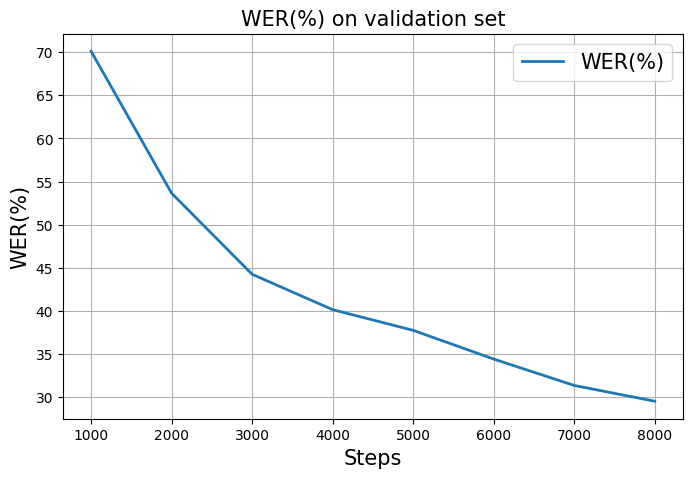
\includegraphics[width=0.8\linewidth, height=0.5\linewidth]{wer-curve.png}
    \caption{WER reduction on validation data during training}
    \label{Fig:WER}

\end{figure}

The initial CNN layers of the transformer for feature extraction are sufficiently trained during pre-training. So during the fine-tuning step we prevent it from further training by freezing their parameters. The hyper-parameters  for fine-tuning are adjusted to obtain the best values. We train our models on a single NVIDIA Tesla T4 GPU using Adam optimiser for 25 epochs. We warm up the learning rate for 800 steps, to a peak of $2.4 \times 10^{−5}$. The trained models are available in Huggingface model hub\footnote{Links will be provided in camera ready paper} along with model cards describing the hyperparameters. We build statistical word level trigram LM using KenLM \cite{heafield2011kenlm} library. The LM is combined with the XLS-R acoustic model using PyCTC decoder.
% The changes we have made to the the default parameter set in CTC layer is tabulated in Table \ref{tab:optimization}. 
% The reduction is word error rate (WER) on validation data during training is illustrated in Fig. \ref{Fig:WER}. 
%, hold for 42000 steps and then exponential decay it

% \begin{table}[htpb]
%     \caption{Hyper-parameters}
%     \label{tab:optimization}
%     \centering
%     \begin{tabular}{ll}
%     \hline \hline
%         \textbf{Parameter} &  \textbf{Values}\\ \hline
%          Attention\_dropout & 0.094 \\
%          Hidden\_dropout & 0.05\\
%          Feat\_proj\_dropout& 0.0 \\
%          Mask\_time\_prob & 0.082 \\
%          % layerdrop & 0.045\\
%          % Update\_freq &\\ 
%          \hline
%     \end{tabular}

% \end{table}

% The reduction in training and validation loss during training process is presented in Fig. \ref{Fig:Trainloss}. 


% \begin{figure}[htpb]
% % \vspace{-0.2}
%     \centering
%     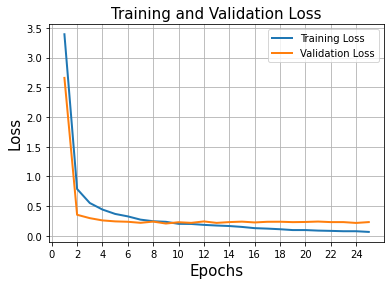
\includegraphics[width=0.8\linewidth, height=0.4\linewidth]{loss.png}
%     \caption{Training and validation loss reduction}
%     \label{Fig:Trainloss}

% \end{figure}



\section{Results and Discussion}

We evaluate our ASR model upon publicly available test datasets, namely T1, T2 and T3 as described in Table \ref{tab:speechdatasets}.  We present the 
results of evaluating our model upon these test datasets, with and without the augmentation of a language model. ASR model performance is measured in terms of word error rate (WER). WER is calculated on the basis of the number of words (N) in the ground truth speech transcript and the number of word insertions (I), deletions (D) and  substitutions (S)  in the  predicted transcript as described in equation \ref{eq:wer}. During evaluation, punctuation have been removed from the ground-truth to ensure no undue penalty is imposed.

\begin{equation}
	\label{eq:wer}
	WER = \frac{(I+D+S) \times 100}{N}
\end{equation}


T1 belongs to the same class of studio recorded read speech corpora used in the training process. T2 and T3 however are OOD datasets, where T3 is particularly unique with its mock conversational nature and noisy recording environments. With a trigram language model on top of XLS-R acoustic model, the WER on the evaluation datasets T1, T2 and T3 are 27.3\%, 37.2\% and 52.9\% respectively. These values show a substantial improvement in WER when compared with the same model without an explicit LM by relative WER reduction of 12.5\%, 15.3\% and 5.9\% respectively.

\begin{figure}[htpb]
% \vspace{-0.2}
    \centering
    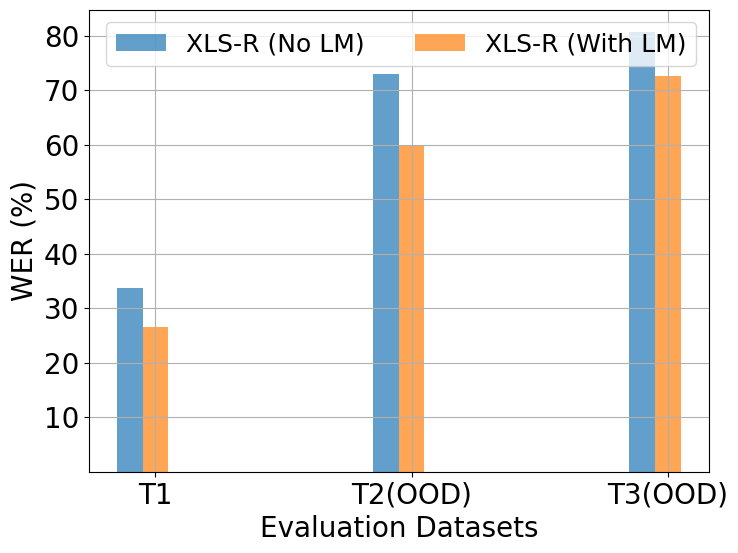
\includegraphics[width=0.55\textwidth]{wer.png}
    \caption{WER on evaluation datasets, with and without LM augmentation}
    \label{Fig:WEReval}

\end{figure}

The resulting WER on different datasets are illustrated in Fig. \ref{Fig:WEReval}. The augmentation of LM clearly shows the possibility of improving ASR systems for morphologically high low resource languages like Malayalam.

% \subsection{Decoding the test speech}

% The decoding process using GMM-HMM and TDNN acoustic models trained with Kaldi requires the use of a language model to aid in the process. We use word-level bigram language models for the same. The GMM-HMM results shown in Table \ref{tab:results} is that of the best triphone acoustic model trained with speaker adaptive training. To decode using the fine-tuned XLS-R model, we use the Viterbi beam search algorithm. We have not used any language model to assist this decoding process.

% \subsection{Performance Evaluation}

% We use two different test datasets as described in section \ref{sec:datasets} to evaluate the models. T1 contains the same domain speech dataset as the train data. It has an OOV rate of 14\%. The OOD test dataset of T2 is has an OOV rate of 44\%.


% \textit{I tested in on google/fleurs test split for Malayalam. Without LM WER = 72.90\%, With LM WER = 60.07\% : Kavya Manohar, June 26 2024
% MSC (without LM) - 86.74\%
% MSC (with LM) - 80.33\% (July 1)
% }

% \begin{table}[!h]
%     \caption{Performance Evaluation}
%     \label{tab:results}
%     \centering
%     \begin{tabular}{l|c|c|c}
%     \hline \hline
%          \textbf{Model}& \multicolumn{3}{c}{\textbf{WER (\%)}} \\  \hline
%            {XLS-R (No LM)}  &{39.8} &{52.5} &{58.87}\\
%          XLS-R (With LM) & & &\\ 
%          \hline
%     \end{tabular}

% \end{table}

\section{Conclusion}

In this work, we have developed an ASR system for the Malayalam language using the self-supervised XLS-R architecture. The transformer is pre-trained on nearly 436K hours of unlabelled multilingual speech and fine-tuned on 69 hours of labelled Malayalam speech data from various publicly available sources. By incorporating a trigram language model on top of the XLS-R transformer, further improvement in the WER by  12.5\% was observed  on in-domain test dataset and an improvement of at least 5.9\% was observed on out-of-domain test datasets. An absolute improvement in WER is expected with additional speech data sources used in the fine-tuning process.


%%%%%%%%%%%%%%%%%%%%%%%%%%%%%%%
%%%%%%%%%%%%%%%%%%%%%%%%%%%%%%%
%   TEMPLATE PART
%%%%%%%%%%%%%%%%%%%%%%%%%%%%%%%
%%%%%%%%%%%%%%%%%%%%%%%%%%%%%%%

% \subsection{A Subsection Sample}
% Please note that the first paragraph of a section or subsection is
% not indented. The first paragraph that follows a table, figure,
% equation etc. does not need an indent, either.

% Subsequent paragraphs, however, are indented.

% \subsubsection{Sample Heading (Third Level)} Only two levels of
% headings should be numbered. Lower level headings remain unnumbered;
% they are formatted as run-in headings.

% \paragraph{Sample Heading (Fourth Level)}
% The contribution should contain no more than four levels of
% headings. Table~\ref{tab1} gives a summary of all heading levels.

% \begin{table}
% \caption{Table captions should be placed above the
% tables.}\label{tab1}
% \begin{tabular}{|l|l|l|}
% \hline
% Heading level &  Example & Font size and style\\
% \hline
% Title (centered) &  {\Large\bfseries Lecture Notes} & 14 point, bold\\
% 1st-level heading &  {\large\bfseries 1 Introduction} & 12 point, bold\\
% 2nd-level heading & {\bfseries 2.1 Printing Area} & 10 point, bold\\
% 3rd-level heading & {\bfseries Run-in Heading in Bold.} Text follows & 10 point, bold\\
% 4th-level heading & {\itshape Lowest Level Heading.} Text follows & 10 point, italic\\
% \hline
% \end{tabular}
% \end{table}


% \noindent Displayed equations are centered and set on a separate
% line.
% \begin{equation}
% x + y = z
% \end{equation}
% Please try to avoid rasterized images for line-art diagrams and
% schemas. Whenever possible, use vector graphics instead (see
% Fig.~\ref{fign}).

% \begin{figure}
% 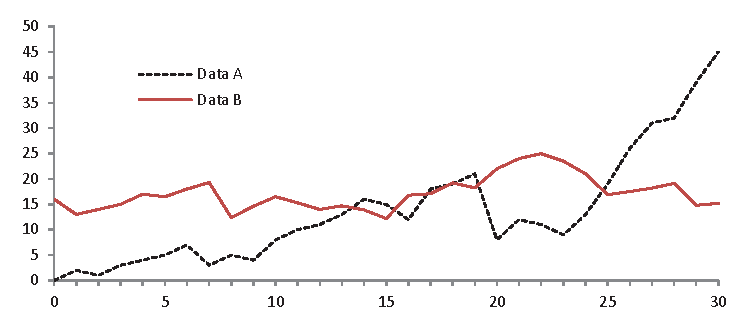
\includegraphics[width=\textwidth]{fig1.eps}
% \caption{A figure caption is always placed below the illustration.
% Please note that short captions are centered, while long ones are
% justified by the macro package automatically.} \label{fign}
% \end{figure}

% \begin{theorem}
% This is a sample theorem. The run-in heading is set in bold, while
% the following text appears in italics. Definitions, lemmas,
% propositions, and corollaries are styled the same way.
% \end{theorem}
% %
% % the environments 'definition', 'lemma', 'proposition', 'corollary',
% % 'remark', and 'example' are defined in the LLNCS documentclass as well.
% %
% \begin{proof}
% Proofs, examples, and remarks have the initial word in italics,
% while the following text appears in normal font.
% \end{proof}
% For citations of references, we prefer the use of square brackets
% and consecutive numbers. Citations using labels or the author/year
% convention are also acceptable. 
% % % The following bibliography provides
% % a sample reference list with entries for journal
% % articles~\cite{ref_article1}, an LNCS chapter~\cite{ref_lncs1}, a
% % book~\cite{ref_book1}, proceedings without editors~\cite{ref_proc1},
% % and a homepage~\cite{ref_url1}. Multiple citations are grouped
% % \cite{ref_article1,ref_lncs1,ref_book1},
% % \cite{ref_article1,ref_book1,ref_proc1,ref_url1}.

% \begin{credits}
% \subsubsection{\ackname} A bold run-in heading in small font size at the end of the paper is
% used for general acknowledgments, for example: This study was funded
% by X (grant number Y).

% \subsubsection{\discintname}
% It is now necessary to declare any competing interests or to specifically
% state that the authors have no competing interests. Please place the
% statement with a bold run-in heading in small font size beneath the
% (optional) acknowledgments\footnote{If EquinOCS, our proceedings submission
% system, is used, then the disclaimer can be provided directly in the system.},
% for example: The authors have no competing interests to declare that are
% relevant to the content of this article. Or: Author A has received research
% grants from Company W. Author B has received a speaker honorarium from
% Company X and owns stock in Company Y. Author C is a member of committee Z.
% \end{credits}
%
% ---- Bibliography ----
%
% BibTeX users should specify bibliography style 'splncs04'.
% References will then be sorted and formatted in the correct style.
%
\bibliographystyle{splncs04}
% \bibliography{mybibliography}
%
\bibliography{refs}

% \begin{thebibliography}{8}
% \bibitem{ref_article1}
% Author, F.: Article title. Journal \textbf{2}(5), 99--110 (2016)

% \bibitem{ref_article1}
% Author, F.: Article title. Journal \textbf{2}(5), 99--110 (2016)

% \bibitem{ref_lncs1}
% Author, F., Author, S.: Title of a proceedings paper. In: Editor,
% F., Editor, S. (eds.) CONFERENCE 2016, LNCS, vol. 9999, pp. 1--13.
% Springer, Heidelberg (2016). \doi{10.10007/1234567890}

% \bibitem{ref_book1}
% Author, F., Author, S., Author, T.: Book title. 2nd edn. Publisher,
% Location (1999)

% \bibitem{ref_proc1}
% Author, A.-B.: Contribution title. In: 9th International Proceedings
% on Proceedings, pp. 1--2. Publisher, Location (2010)

% \bibitem{ref_url1}
% LNCS Homepage, \url{http://www.springer.com/lncs}, last accessed 2023/10/25
% \end{thebibliography}
\end{document}
